\section{Problemformulering}
Tracking af en lerdue i English Skeet (ES) vha. PTS. 
Lerduen er i vores opstilling udskiftet med en bold, men ellers følges reglerne for ES, \citep{ES_regler}.
Bolden bevæger sig i et 3D-rum med negligerbar luftmodstand. \\

\begin{figure}[th!]
\centering
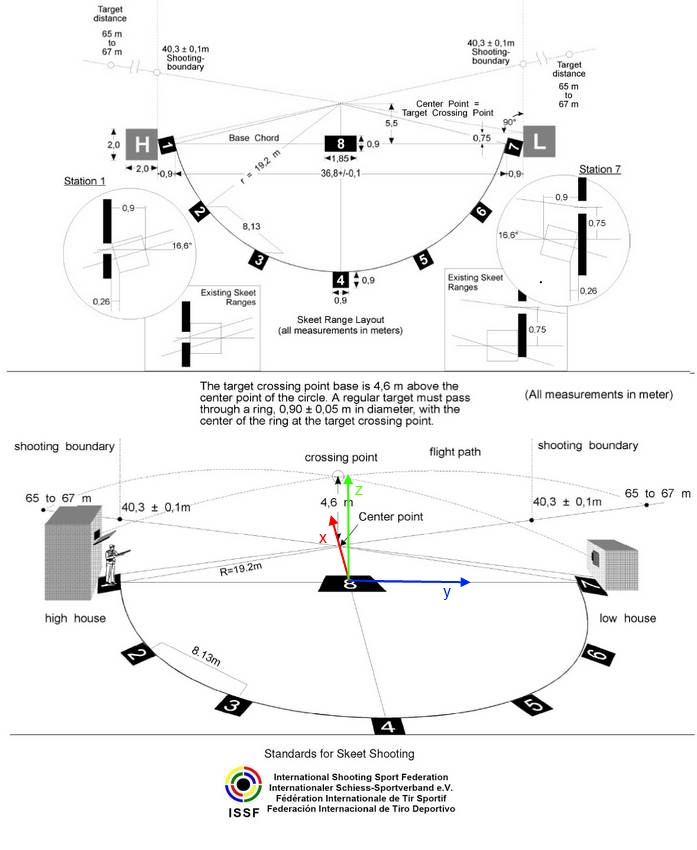
\includegraphics[width=0.4\textwidth]{./graphics/skeet-diagram_med_akser}
\caption[tekst i indholdsfortegnelsen]{figurtekst}
\label{fig:ES}
\end{figure}	
Systemets input er 60 kartesisiske koordinatsæt (x,y,z) per sekund. Hvor disse 
koordinater stammer fra, er uden for projektafgrænsningen. \\

Systemet dimensioneres til brug ifbm. en konkurrence i ES. En skitse over 
banen ses på figur \ref{fig:ES}. Det kartesiske koordinatsystem har origo i halvcirklens centrum, 
som indtegnet 
nederst på figuren. I ES skal rammes serier af duer/mål der afskydes fra 
enten ”High House” eller ”Low House”, og med skud fra hver af de otte stationer langs 
cirkelperiferien. Dette projekt er afgrænset til et enkelt tilfælde - afskydning fra ”High-
House” med pan-and-tilt systemet placeret på station 4.\\

Jævnfør reglerne for ES, skal duer/mål passere target crossing point (TCS) som er 
placeret i $4,57 [m]$ over origo. (0; 0; 4.57). Fejlmargin for passagen er $\pm0,45 [m]$. 
Målene skal desuden flyve $50 - 52 [m]$.  High house er placeret $20,11 [m]$ fra TCS, i en 
højde af $3,05 [m]$. 
%Da luftmodstanden er negligerbar kan parablen (2. grads polynomium) findes ved at indsætte de kendte punkter. 
Herunder er parablen vist i et 
2D plan, figur \ref{fig:HH2D_para}.
\begin{figure}[!th]
\centering
\begin{tikzpicture}[scale=1]
\include*{./graphics/high_house_2D_parabola}
\end{tikzpicture}
\caption[Lerdue parabel]{Viser parablen af lerduens bane i 2D}
\label{fig:HH2D_para}
\end{figure}
~\\[10pt]
Målet bliver affyret med en hastighed på $34.589 [\frac{m}{s}]$, i en vinkel på $9.103^{\circ}$ ift. xy-
planet. Set ovenfra bevæger målet sig som set på figur \ref{fig:para_in_xy_plane}. 
Figuren ses nedslagspunktet fra High-House, der er i alt $52 [m]$ startpositionen samt 
PTS placering i punktet B. 



\begin{figure}[!th]
\centering
\begin{tikzpicture}[scale=0.2]
\include*{./graphics/parabola_in_xy_plane}
\end{tikzpicture}
\caption[tekst i indholdsfortegnelsen]{Viser målets bane set ovenfra. D er udgangspunktet, G er nedslagspunktet. B er placeringen af PTS.}
\label{fig:para_in_xy_plane}
\end{figure}

\subsection{Udregning af tallene}
\todo[inline, author=Michael]{Skal sikkert flyttes til appendix?}

For at simplificere udregningerne, regnes parablen kun i 2D. Det er trivielt at tilføje den tredje, så det gøres til sidst (hvis jeg finder det relevant). 

Kasteparablen er givet ved vektorfunktionen i ligning  \ref{eq:pf:vektorparabel}.

\begin{equation}
	Pos(t) = \left( \begin{array}{c}
	x_{2D}(t) \\
	y_{2D}(t)
	\end{array}
	\right)
	= \left( \begin{array}{c}
	\cos \theta v_0 t + x_0 \\
	\sin \theta v_0 t - \frac{g}{2} t^2 + y_0
	\end{array}
	\right)
\label{eq:pf:vektorparabel}
\end{equation}

Hvor $\theta$ er afskydningsvinklen, $v_0$ er afskydningshastigheden, $g$ er tyngdeacceleration og $x_0$,$y_0$ er begyndelsespunktet. 

For at få en parabel på formen y(x), isoleres t i x(t) med henblik på at substituere t i y(x): ($x_0$ sættes til 0.)

\begin{equation}
t = \frac{x}{\cos \left( \theta \right) v_0}
\label{eq:pf:x(t)}
\end{equation}

Den fundne værdi for t indsættes i $y(t)$, og udtrykket reduceres, \citep[Side. 67]{fund_of_physics}: 

\begin{align}
\begin{split}
y(t(x)) &= \sin \left( \theta \right) \frac{x}{\cos \left( \theta \right) v_0} v_0 - \frac{g}{2} \left(\frac{x}{\cos \left( \theta \right) v_0}\right)^2 + y_0 \\
y(x) &= \tan \left( \theta \right) x - \frac{gx^2}{2(\cos \left( \theta \right) v_0)^2} + y_0
\label{eq:pf:y(x(t))}
\end{split}
\end{align}

Det ses at der er 3 ubekendte i ligningen. Dog er 3 punkter kendt fra HH parablen. Det er givet i reglerne for ESS at målet affyres fra en højde på $y_0 = 3.05 [m]$, så det indsættes i formlen. 
\begin{equation}
y(x) = \tan \theta x - \frac{gx^2}{2(\cos \left( \theta \right)  v_0)^2} + 3.05
\label{eq:pf:y(x)2}
\end{equation}
Det er givet at målet skal passere TCS som er placeret i en højde på $4.57 [m]$, $20.11 [m$] fra HH. 
Desuden skal målet bevæge sig $50 - 52 [m]$, i de videre beregninger $52 [m]$. Det giver koordinatsættene (20.11; 4.57) og (52; 0). Vha. disse bestemmes $\theta$ og $v_0$ til:\footnote{Ved $g = 9.82[m/{s}^{2]}$}
\todo[inline, author=Michael]{Måske giver det ikke mening med alle de decimaler, da det er udregnet med g = 9.82 - men jeg ved heller ikke hvor jeg skal finde en mere præcis måling af g?}
\begin{eqnarray}
\theta &=& 9.103 \degree \\
v_0 &=& 34.589 \left[ \frac { m }{ s }  \right] 
\end{eqnarray}

Disse parametre indsættes i vektorfunktionen fra ligning \ref{eq:pf:vektorparabel} samt udtrykket fra ligning \ref{eq:pf:y(x)2}. Udtrykkene reduceres: 

\begin{align}
\begin{split}
	Pos(t) = \left( \begin{array}{c}
	x_{2D}(t) \\
	y_{2D}(t)
	\end{array}
	\right)
	&= \left( \begin{array}{c}
	\cos \left(9.103 \degree \right) 34.589 t \\
	\sin \left(9.103 \degree \right) 34.589 t - \frac{9.82}{2} t^2 + 3.05
	\end{array}
	\right) \\
% ------------------------------
	&= \left( \begin{array}{c}
	34.153 t \\
	- 4.91 t^2 + 5.473 t + 3.05
	\end{array}
	\right)
\label{eq:pf:vektorparabel2}
\end{split}
\end{align}

\begin{align}
\begin{split}
y(x) &= \tan \left(9.103 \degree \right) x - \frac{9.82x^2}{2(\cos \left(9.103 \degree \right) 34.589)^2} + 3.05 \\
% -------------------------------
&= - 0.00421 x^2 + 0.1602 x  + 3.05
\label{eq:pf:y(x)3}
\end{split}
\end{align}

For at finde ud af hvornår målet rammer jorden, sættes $y(t) = 0$. Det giver:

\begin{equation}
t_{nedslag} = 1.523 [s]
\label{eq:pf:nedslagstid}
\end{equation}

\subsubsection{Parabel i 3 dimensioner}
Nu omskrives parablen fundet i \ref{eq:pf:vektorparabel2} til x,y,z koordinater. 
Grundplanet er x,y og højden er givet ved z. Dvs. at $z(t) = y_{2D}(t)$ og at $x(t)$ samt $y(t)$ afhænger af $x_{2D}(t)$ samt vinklen $\alpha$. 
$\alpha$ er givet ved vinklen mellem parablen projekteret ned på x,y planet (som på figur \ref{fig:para_in_xy_plane}) og x aksen. 
\todo[inline, author=Michael, color=blue! 50]{Kan også skrives som vinklen mellem parablen og x,z planet?}
Vektorfunktionen kan skrives (ved $\alpha = 15.872 \degree$): 

\begin{align}
\begin{split}
Pos(t) = \left( \begin{array}{c}
	x(t) \\
	y(t) \\
	z(t)
	\end{array}
	\right)
%----------------------------------------
	&= \left( \begin{array}{c}
	\cos \alpha \times x_{2D}(t) - 19.3 \\
	\sin \alpha \times x_{2D}(t) - 5.5 \\
	y_{2D}(t)
	\end{array}
	\right) \\
%----------------------------------------
	&= \left( \begin{array}{c}
	32.851 t - 19.3 \\
	9.34 t - 5.5 \\
	- 4.91 t^2 + 5.473 t + 3.05
	\end{array}
	\right)
\label{eq:pf:vektorparabel3d}
\end{split}
\end{align}


Bemærk udgangspunktet for kastet er flyttet fra origo, til HHs position. (Punkt D på figur \ref{fig:para_in_xy_plane})
